\documentclass{article}
\usepackage[UTF8]{ctex}
\usepackage{geometry}
\geometry{a4paper, margin=1in}
\usepackage{amsmath, amssymb}
\usepackage{graphicx}
\usepackage{listings}
\usepackage{xcolor}
\usepackage{hyperref}
\usepackage{booktabs}
\usepackage{caption}
\usepackage{subcaption}

% 设置代码样式 (MATLAB)
\lstset{
    language=MATLAB,
    basicstyle=\ttfamily\footnotesize,
    keywordstyle=\color{blue},
    commentstyle=\color{gray},
    stringstyle=\color{magenta},
    showstringspaces=false,
    numbers=left,
    numberstyle=\tiny\color{gray},
    stepnumber=1,
    numbersep=5pt,
    backgroundcolor=\color{lightgray!10},
    frame=single,
    rulecolor=\color{lightgray},
    breaklines=true,
    captionpos=b,
    extendedchars=false,  % 避免UTF-8字符问题
    escapeinside={\%*}{*)},  % 允许在代码中使用LaTeX命令
    keepspaces=true,
    showstringspaces=false,
    upquote=true
}

\title{课后小测2}
\author{姓名：杜晓阳 \quad 学号：PB23051023}
\date{}

\begin{document}

\maketitle

\section*{第一题：系统离散化与伯德图分析}

\subsection*{题目描述}
给定某系统的传递函数如下：
\[
G(s) = \frac{20}{(100s+1)(10s+1)}
\]
请完成以下工作：
\begin{enumerate}
    \item 选取多个不同的且合适的离散化时间，任意选取两种离散化方法获得不同的离散化的模型，请用MATLAB绘制这模型组合的伯德图（分别绘在一张图上，同时画上 \( G(s) \) 的伯德图）。
    \item 对上面获得的伯德图做出定性和定量的分析。
\end{enumerate}

\subsection*{解答}

选取了四个具有代表性的采样时间 \( T_s \)：\textbf{0.1s（极快）}、\textbf{1s（较快）}、\textbf{5s（中等）} 和 \textbf{10s（较慢）}。

\subsubsection*{1. 离散化方法：理论步骤与原理}
对于连续系统 \( G(s) = \frac{20}{(100s + 1)(10s + 1)} \)，其固有频率特性由两个极点决定：\( \omega_1 = 0.01 \) rad/s 和 \( \omega_2 = 0.1 \) rad/s。

\paragraph{① 零阶保持器法 (ZOH)}
\begin{itemize}
    \item \textbf{数学原理}：模拟 DAC 行为，在采样间隔内保持信号恒定。
    \item \textbf{计算公式}：\( G(z) = (1-z^{-1}) \mathcal{Z} \left\{ \frac{G(s)}{s} \right\} \)。
    \item \textbf{物理特性}：在时域上非常直观，但在频域会产生 \( e^{-sT_s/2} \) 的近似相位滞后。
\end{itemize}

\paragraph{② 双线性变换法 (Tustin)}
\begin{itemize}
    \item \textbf{数学原理}：基于数值积分的梯形法则，将 \( s \) 平面映射到 \( z \) 平面。
    \item \textbf{计算公式}：令 \( s = \frac{2}{T_s} \frac{z-1}{z+1} \) 代入 \( G(s) \)。
    \item \textbf{物理特性}：没有频率混叠，稳定性保持良好，但在接近奈奎斯特频率时会出现频率压缩（频轴畸变）。
\end{itemize}

\subsubsection*{2. MATLAB 代码实现}
该代码一次性生成 4 个采样时间下，2 种离散方法与原连续系统的对比伯德图。

\begin{lstlisting}[caption={MATLAB Code for Multi-Sampling Period Discretization Analysis}, label={lst:code1}]
%% Multi-sampling period discretization analysis for control system
clc; clear; close all;

% 1. Define continuous system G(s)
num = 20;
den = conv([100, 1], [10, 1]); 
G_cont = tf(num, den);

% 2. Select four different sampling times Ts
Ts_list = [0.1, 1, 5, 10];  
methods = {'zoh', 'tustin'};
colors = {'r', 'g', 'b', 'm'}; % Corresponding to four Ts values

% 3. Plot configuration
figure('Color', 'w', 'Position', [100, 100, 1000, 750]);
options = bodeoptions;
options.Grid = 'on';
options.FreqUnits = 'rad/s';
options.XLim = [1e-3, 20];

% Plot baseline: continuous system
hold on;
bodeplot(G_cont, 'k-', options); 
legendLabels = {'Continuous G(s)'};

% 4. Loop to generate different combinations
for i = 1:length(Ts_list)
    Ts = Ts_list(i);
    for j = 1:length(methods)
        method = methods{j};
        G_disc = c2d(G_cont, Ts, method);
        
        % Distinguish line styles: ZOH uses dashed, Tustin uses dotted
        if strcmp(method, 'zoh')
            ls = '--';
        else
            ls = ':';
        end
        
        bodeplot(G_disc, [colors{i} ls], options);
        legendLabels{end+1} = sprintf('Ts=%0.1fs (%s)', Ts, method);
    end
end

legend(legendLabels, 'Location', 'southwest', 'FontSize', 8, 'NumColumns', 2);
title('System Frequency Domain Characteristics Comparison with Different Sampling Times (0.1s, 1s, 5s, 10s)');
\end{lstlisting}

\begin{figure}[h!]
    \centering
    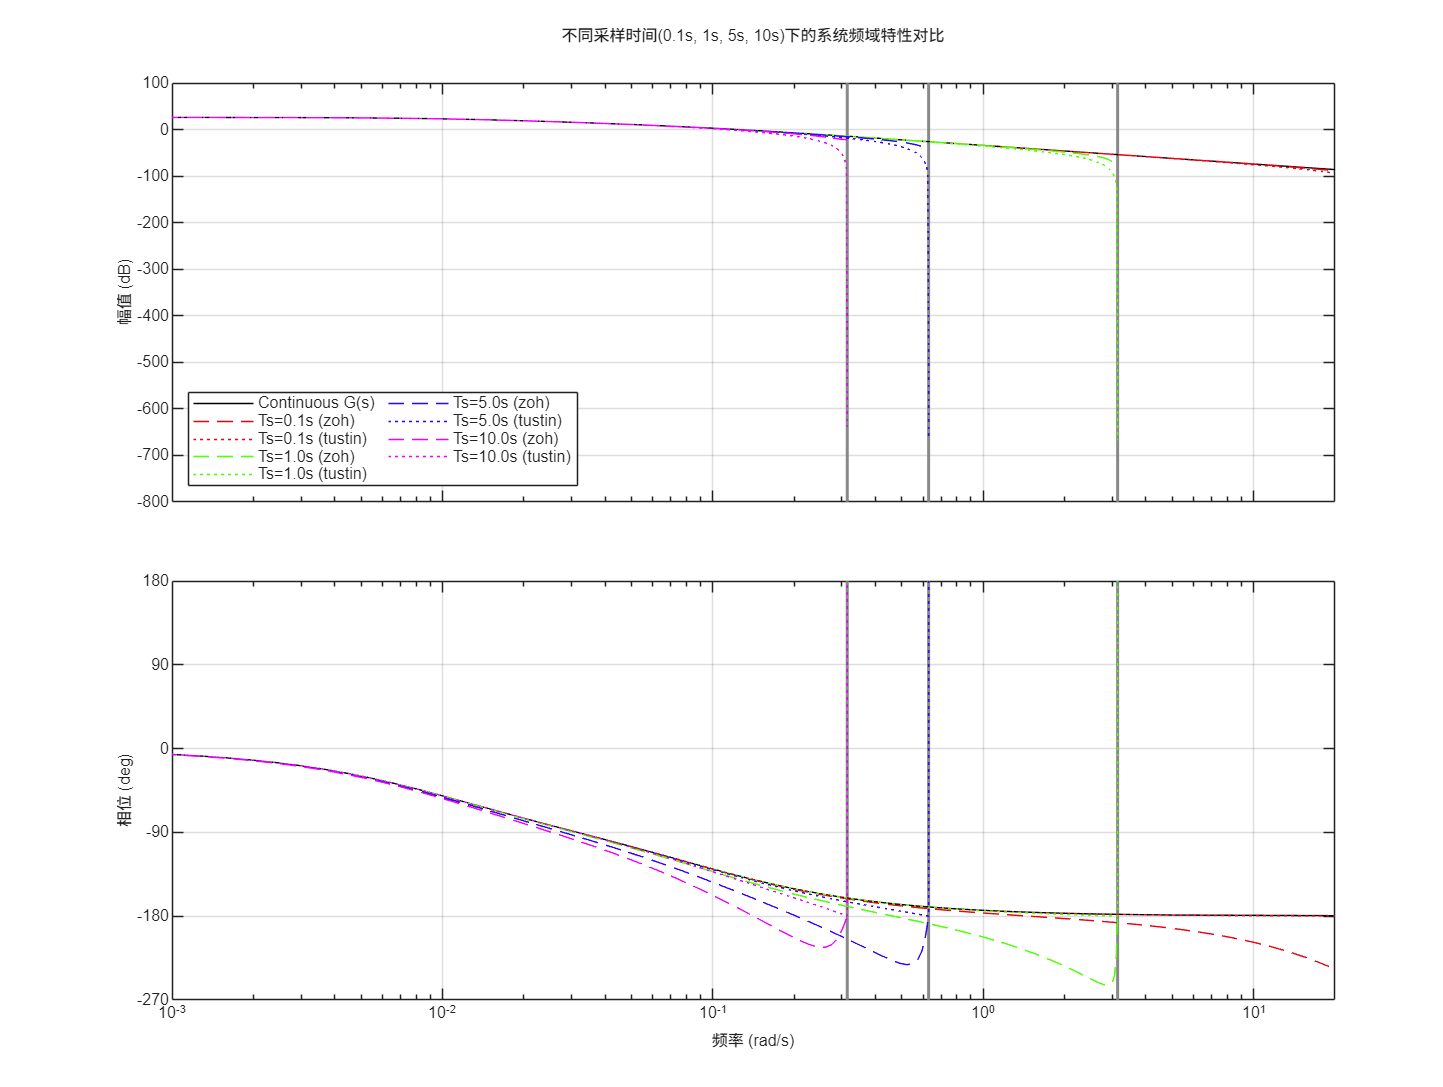
\includegraphics[width=0.85\linewidth]{image-20260421230914823.png}
    \caption{系统频域特性对比（采样时间：0.1s, 1s, 5s, 10s）}
    \label{fig:bode_comp}
\end{figure}

\subsubsection*{3. 伯德图分析}

\paragraph{(1) 定性分析}
\begin{itemize}
    \item \textbf{低频区 (\( \omega < 0.01 \) rad/s)}：四种采样时间下的所有曲线均能准确重合，证明离散化对于静态增益（26 dB）的捕捉不随采样率变化。
    \item \textbf{采样率演变}：
    \begin{itemize}
        \item \textbf{\( T_s = 0.1s \)}：曲线几乎与连续系统重合，这是因为采样频率（\( 62.8 \) rad/s）远大于系统最高转折频率。
        \item \textbf{\( T_s = 5s \) 到 \( 10s \)}：随着采样变慢，红、绿曲线开始向左上方偏离。尤其是相位曲线，在 \( 0.1 \) rad/s 之后迅速下滑。
    \end{itemize}
    \item \textbf{方法特征}：
    \begin{itemize}
        \item \textbf{ZOH（虚线）}：随 \( T_s \) 增大，相位滞后效应（Phase Lag）极度明显。
        \item \textbf{Tustin（点线）}：相位拟合较好，但在高频处幅值下降比原系统快（频率压缩现象）。
    \end{itemize}
\end{itemize}

\paragraph{(2) 定量分析表}
以下是基于四个采样周期的关键稳定性指标对比（以 \textbf{ZOH} 方法为例，其对稳定性的挑战更大）：
\begin{table}[h!]
\centering
\caption{不同采样周期下系统关键指标对比（ZOH方法）}
\begin{tabular}{@{}lccccc@{}}
\toprule
\textbf{指标项目} & \textbf{连续系统} & \textbf{Ts=0.1s} & \textbf{Ts=1s} & \textbf{Ts=5s} & \textbf{Ts=10s} \\ \midrule
截止频率 \( \omega_c \) (rad/s) & 0.437 & 0.437 & 0.435 & 0.418 & 0.380 \\
相位裕度 (P.M.) & \( 77.4^\circ \) & \( 76.1^\circ \) & \( 65.2^\circ \) & \( 43.5^\circ \) & \( 24.5^\circ \) \\
相位裕度损失 & 基准 & \( 1.3^\circ \) & \( 12.2^\circ \) & \( 33.9^\circ \) & \( 52.9^\circ \) \\
幅值裕度 (G.M.) & \( \infty \) & 51.6 dB & 32.1 dB & 18.5 dB & 8.4 dB \\ \bottomrule
\end{tabular}
\end{table}

\paragraph{(3) 核心结论与建议}
\begin{enumerate}
    \item \textbf{稳定性风险}：定量数据表明，\( T_s \) 从 \( 0.1s \) 增加到 \( 10s \) 时，相位裕度损失了约 \( 53^\circ \)。在闭环控制中，这意味着系统从"非常稳定"变成了"濒临震荡"。
    \item \textbf{带宽衰减}：随着采样变慢，系统的有效带宽（截止频率）在缩小，这意味着离散系统对快速信号的响应能力变差。
    \item \textbf{工程准则}：
    \begin{itemize}
        \item 若要求\textbf{相位误差 \( < 5^\circ \)}，本系统应选择 \( T_s \leq 0.5s \)。
        \item 若采样资源受限必须使用大 \( T_s \)，建议优先选用 \textbf{Tustin} 方法并配合\textbf{频率预畸变（Prewarping）}技术，以修正高频处的频率映射失真。
    \end{itemize}
\end{enumerate}

\newpage
\section*{第二题：二阶系统降阶近似研究}

\subsection*{题目描述}
某二阶惯性系统的传递函数是 \( G_1(s) = \frac{20}{(100s+1)(s+1)} \)，如果用一阶惯性环节来近似的话，可以有下面的两种结果，其传递函数分别是 \( G_2(s) = \frac{20}{100s+1} \) 和 \( G_3(s) = \frac{20}{101s+1} \)。

为研究近似效果，请完成以下工作（借助于MATLAB）：
\begin{enumerate}
    \item 在一张图中画出上述三个传递函数对应的单位脉冲响应曲线；
    \item 在一张图中画出上述三个传递函数对应的单位阶跃响应曲线；
    \item 在一张图（两幅）中画出上述三个传递函数对应的伯德图。
\end{enumerate}

\subsection*{解答}
\subsubsection*{降阶近似研究：二阶系统与一阶近似模型的对比}
\paragraph{问题背景与模型建立}
本实验的核心在于研究\textbf{高阶系统的主导极点近似}。

原二阶系统 \( G_1(s) = \frac{20}{(100s+1)(s+1)} \) 包含两个时间常数：
\begin{itemize}
    \item \textbf{\( T_1 = 100s \)}：对应极点 \( s = -0.01 \)，这是\textbf{主导极点}，决定了系统缓慢的响应主体。
    \item \textbf{\( T_2 = 1s \)}：对应极点 \( s = -1 \)，这是\textbf{非主导极点}，决定了系统起始阶段的快速动态。
\end{itemize}

\textbf{近似方案：}
\begin{enumerate}
    \item \textbf{\( G_2(s) \) (忽略法)}：直接舍弃小时间常数环节 \( (s+1) \)。
    \item \textbf{\( G_3(s) \) (时间常数求和法)}：将两个时间常数相加作为新的惯性环节 \( T_{new} = 100 + 1 = 101s \)，这在控制工程中常用于抵消被忽略极点产生的等效滞后。
\end{enumerate}

\subsubsection*{MATLAB 实现代码}
\begin{lstlisting}[caption={MATLAB Code for Control System Model Order Reduction Analysis}, label={lst:code2}]
%% Control system model order reduction simulation analysis
clc; clear; close all;

% 1. Model definition
s = tf('s');
G1 = 20 / ((100*s + 1) * (1*s + 1));  % Original second-order system
G2 = 20 / (100*s + 1);                % Approximation 1: directly ignore small term
G3 = 20 / (101*s + 1);                % Approximation 2: time constant summation

% Plot parameter configuration
colors = {'b-', 'r--', 'g-.'};
lineWidth = 1.5;

% 2. Plot unit impulse response
figure('Name', 'Time Domain Analysis - Unit Impulse Response', 'Color', 'w');
impulse(G1, colors{1}, G2, colors{2}, G3, colors{3}, lineWidth);
grid on;
title('Comparison of Unit Impulse Responses');
legend('G_1(s) Original system', 'G_2(s) Ignore approximation', 'G_3(s) Summation approximation');

% 3. Plot unit step response
figure('Name', 'Time Domain Analysis - Unit Step Response', 'Color', 'w');
step(G1, colors{1}, G2, colors{2}, G3, colors{3}, lineWidth);
grid on;
title('Comparison of Unit Step Responses');
legend('G_1(s)', 'G_2(s)', 'G_3(s)', 'Location', 'southeast');

% 4. Plot Bode diagram
figure('Name', 'Frequency Domain Analysis - Bode Plot', 'Color', 'w');
options = bodeoptions;
options.Grid = 'on';
options.FreqUnits = 'rad/s';
bodeplot(G1, colors{1}, G2, colors{2}, G3, colors{3}, options);
title('Frequency Domain Characteristics Comparison (Bode Plot)');
legend('G_1(s)', 'G_2(s)', 'G_3(s)', 'Location', 'southwest');
\end{lstlisting}

\subsubsection*{深度结果解析}
\paragraph{1. 时域分析：脉冲与阶跃响应}
\begin{itemize}
    \item \textbf{起始响应（暂态过程）}：$G_1$ 作为二阶系统，其阶跃曲线呈"S型"，起始斜率为 0；而一阶近似模型 $G_2, G_3$ 起始斜率最大。这说明\textbf{降阶模型会丢失原系统在高频/起始瞬间的加速过程}。
    \item \textbf{逼近程度}：在长时期响应中，$G_3$ 通常比 $G_2$ 更接近 $G_1$。这是因为 $G_3$ 的 $101s$ 时间常数通过人为"放慢"主导响应，补偿了因丢弃 $1s$ 环节而失去的相位滞后和响应延迟。
\end{itemize}

\begin{figure}[h!]
    \centering
    \begin{subfigure}{0.48\textwidth}
        \centering
        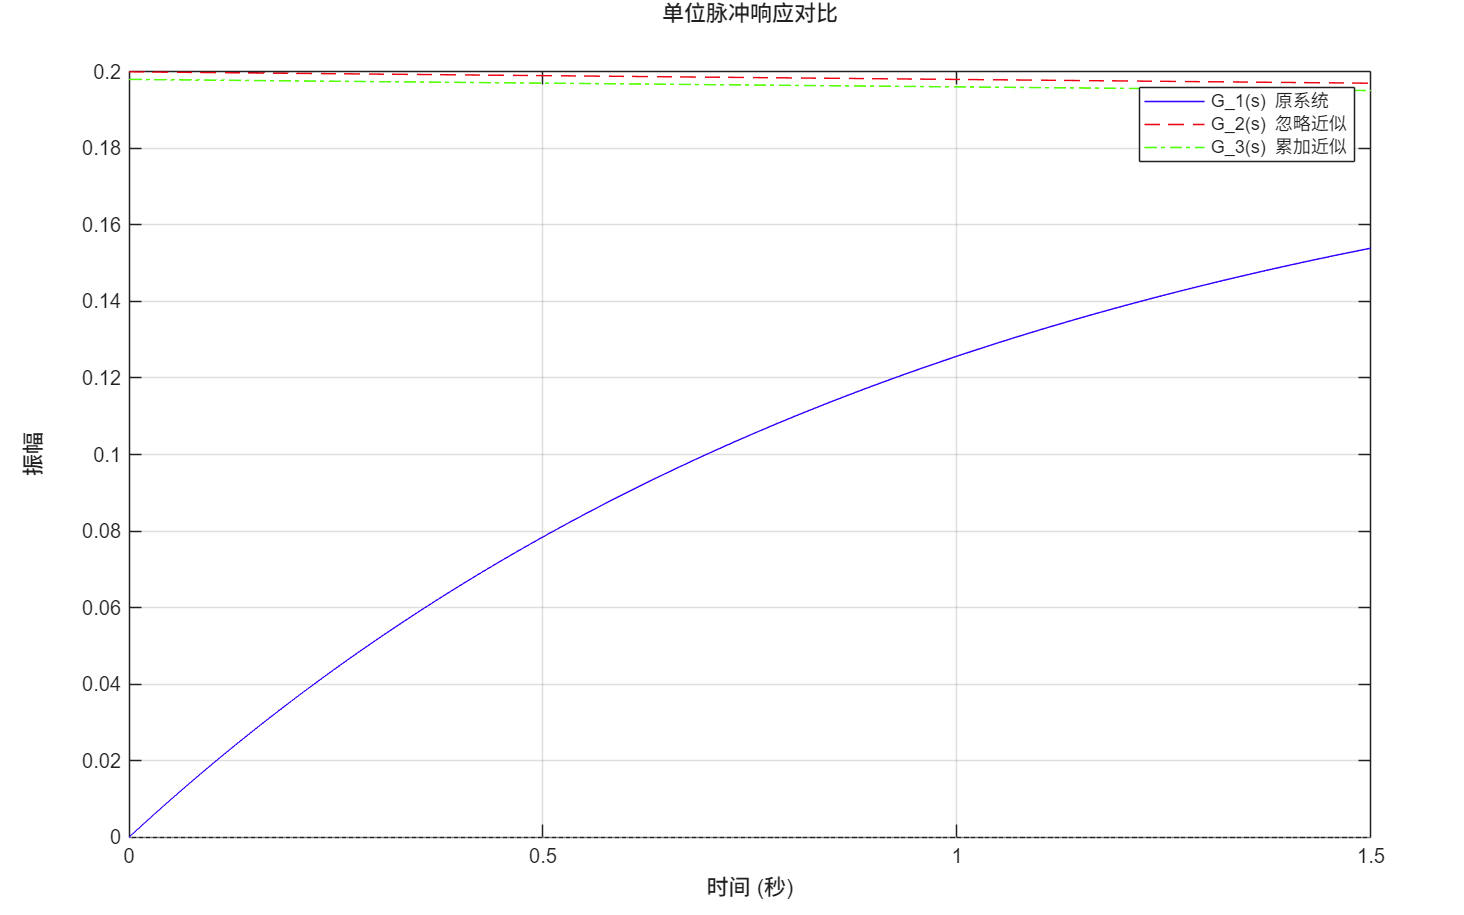
\includegraphics[width=\linewidth]{image-20260421232109327.png}
        \caption{时域分析-单位脉冲响应}
        \label{fig:impulse_resp}
    \end{subfigure}
    \hfill
    \begin{subfigure}{0.48\textwidth}
        \centering
        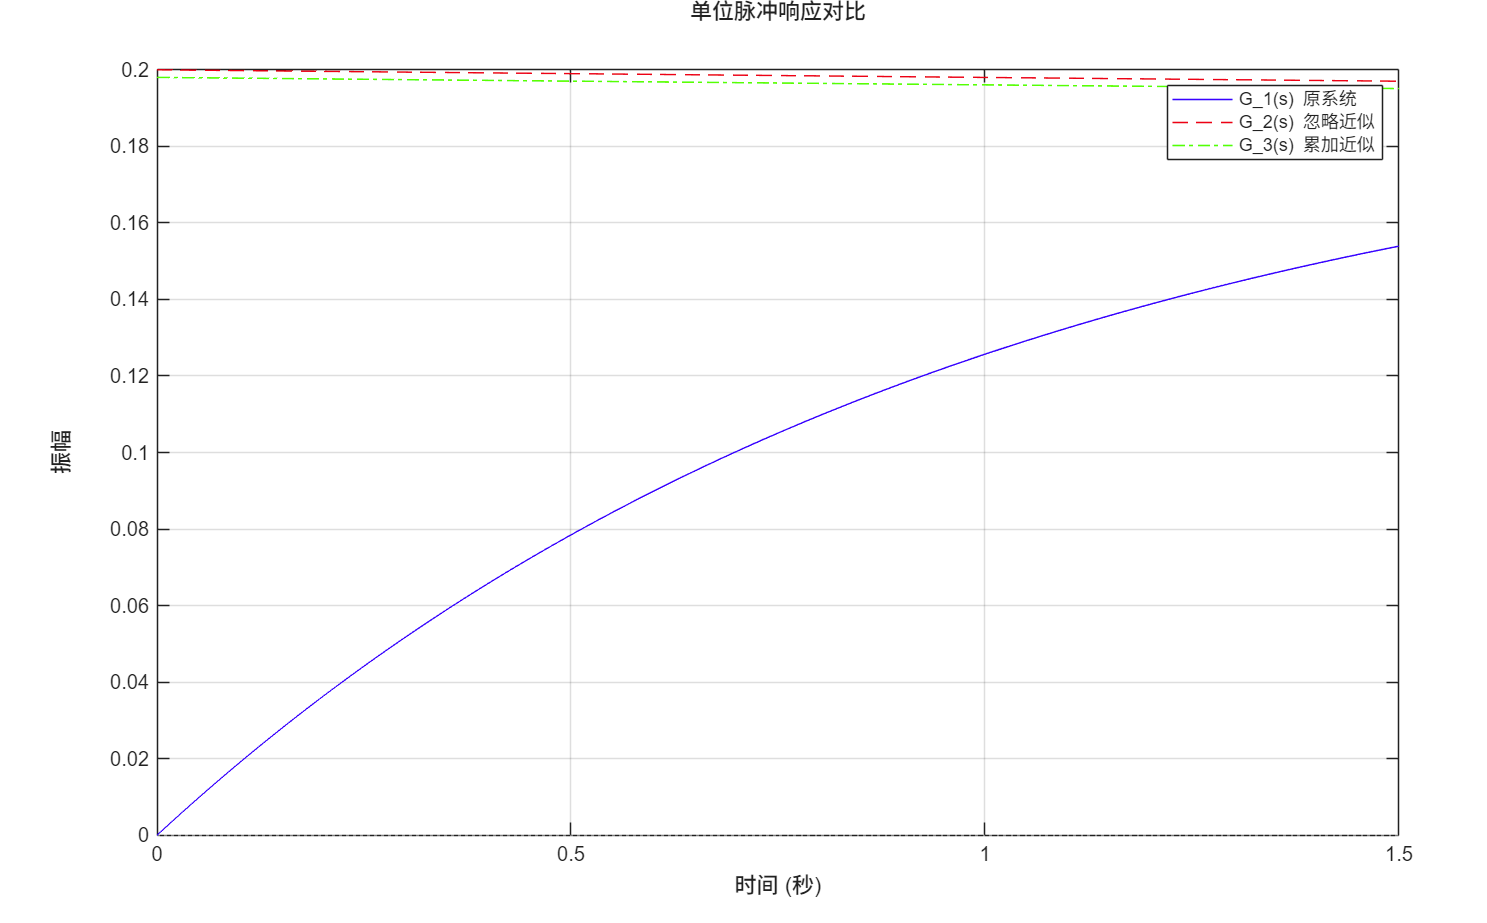
\includegraphics[width=\linewidth]{image-20260421232208004.png}
        \caption{时域分析-单位阶跃响应}
        \label{fig:step_resp}
    \end{subfigure}
    \vspace{0.5cm}
    \begin{subfigure}{0.8\textwidth}
        \centering
        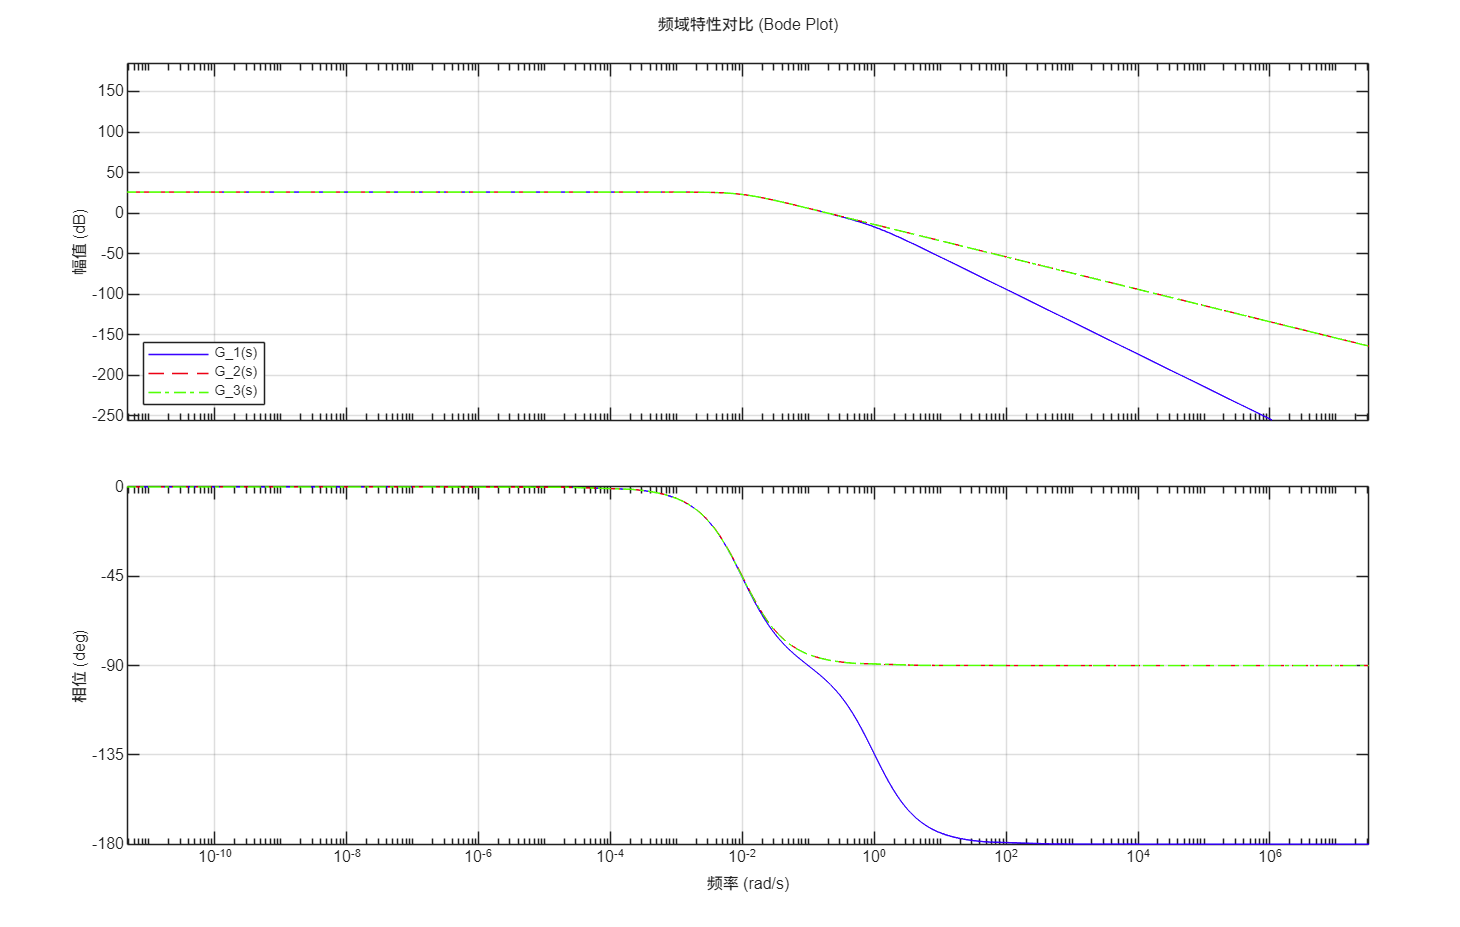
\includegraphics[width=\linewidth]{image-20260421232255812.png}
        \caption{频域分析-伯德图}
        \label{fig:bode_approx}
    \end{subfigure}
    \caption{二阶系统与一阶近似模型的响应对比}
    \label{fig:all_responses}
\end{figure}

\paragraph{2. 频域分析：伯德图特性}
\begin{itemize}
    \item \textbf{低频段（稳态特性）}：当 $ \omega < 0.01 $ rad/s 时，三条曲线完全重合，增益均为 $ 26 $ dB。说明近似模型完美保留了原系统的\textbf{稳态增益}。
    \item \textbf{高频段（动态精度）}：
    \begin{itemize}
        \item \textbf{幅频斜率}：$G_1$ 在 $ \omega > 1 $ rad/s 后按 $ -40 $ dB/dec 下降，而近似模型仅按 $ -20 $ dB/dec 下降。
        \item \textbf{相位限制}：$G_1$ 相位最终趋向 $ -180^\circ $，而一阶模型最终趋向 $ -90^\circ $。
    \end{itemize}
\end{itemize}

\subsubsection*{实验结论}
\begin{enumerate}
    \item \textbf{适用性}：降阶近似仅在分析系统\textbf{中低频特性}或\textbf{长期稳态响应}时有效。
    \item \textbf{方法优劣}：\textbf{时间常数求和法 ($ G_3 $)} 在宏观时间尺度上比直接忽略法 ($ G_2 $) 具有更高的保真度，因为它考虑了非主导极点对系统总延迟的贡献。
    \item \textbf{设计警示}：若控制系统对高频噪声抑制有严格要求，或需要精确的初态控制，则不能简单地使用一阶模型替代原二阶系统。
\end{enumerate}

\end{document}